\documentclass[a4paper,ngerman,12pt]{scrartcl}

\usepackage[utf8]{inputenc}
%\usepackage[ansinew]{inputenc}

\usepackage[ngerman]{babel}

\usepackage{amsmath,amsthm,amssymb,stmaryrd,color,graphicx}
\usepackage{setspace}
\usepackage{bussproofs}
\usepackage{array}
\usepackage{comment}
\usepackage{wrapfig}

\usepackage{enumitem}

\usepackage{siunitx}

\usepackage[protrusion=true,expansion=true]{microtype}

\usepackage{lmodern}

\usepackage{hyperref}
\usepackage{cleveref}

\newcommand{\RR}{\mathbb{R}}
\newcommand{\CC}{\mathbb{C}}
\newcommand{\ZZ}{\mathbb{Z}}
\newcommand{\NN}{\mathbb{N}}
\newcommand{\QQ}{\mathbb{Q}}

\setlength\parskip{\medskipamount}
\setlength\parindent{0pt}

\theoremstyle{definition}
\newtheorem{defn}{Definition}[]
\newtheorem{axiom}[defn]{Axiom}
\newtheorem{bsp}[defn]{Beispiel}

\theoremstyle{plain}
\newtheorem{prop}[defn]{Proposition}
\newtheorem{motto}[defn]{Motto}
\newtheorem{wunder}[defn]{Wunder}
\newtheorem{ueberlegung}[defn]{Überlegung}
\newtheorem{lemma}[defn]{Lemma}
\newtheorem{kor}[defn]{Korollar}
\newtheorem{hilfsaussage}[defn]{Hilfsaussage}
\newtheorem{satz}[defn]{Satz}
\newtheorem{frage}[defn]{Frage}

\theoremstyle{remark}
\newtheorem{bem}[defn]{Bemerkung}
\newtheorem{aufg}[defn]{Aufgabe}

\newtheorem*{antwort}{Antwort}

\newlength{\aufgabenskip}
\setlength{\aufgabenskip}{1.4em}
\newcounter{aufgabennummer}
\newenvironment{aufgabe}[1]{
	\refstepcounter{aufgabennummer}
	\textbf{Aufgabe \theaufgabennummer.} \emph{#1} \par
}{\vspace{\aufgabenskip}}
\crefname{aufgabennummer}{Aufgabe}{Aufgaben}
\Crefname{aufgabennummer}{Aufgabe}{Aufgaben}

\clubpenalty=10000
\widowpenalty=10000
\displaywidowpenalty=10000

\setlength\unitlength{1cm}

\usepackage{tikz}

\RequirePackage{geometry}
\geometry{textwidth=16.0cm,textheight=24.5cm,footskip=1.5cm}

\usepackage{todonotes}


\begin{document}
	
\begin{picture}(0,0)
\put(0,-0.5){%
	
\includegraphics[scale=0.1]{logo-ifm}
}
\put(14.0,-3.5){%
	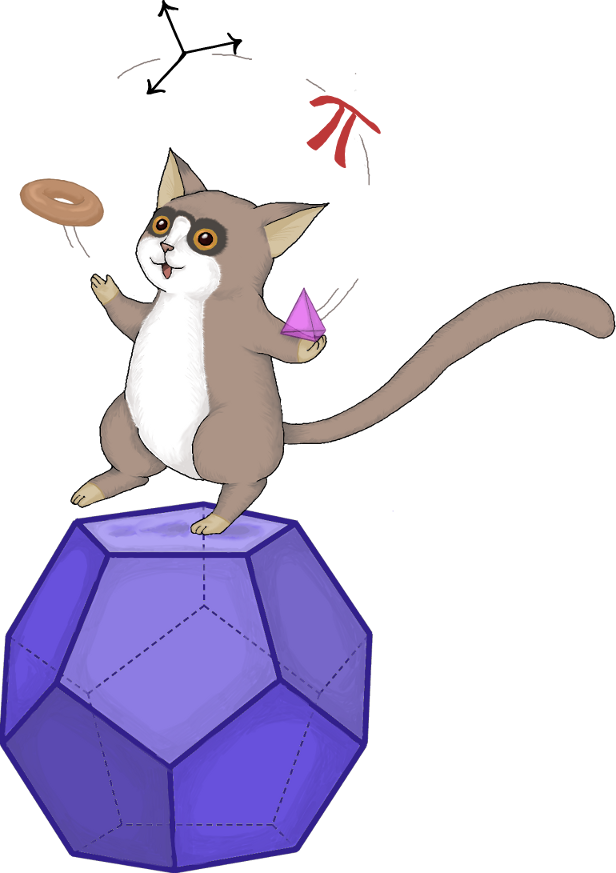
\includegraphics[scale=0.17]{cover}
}
\end{picture} 
	
\vspace{6em}

\begin{center}\Large{Vierter Korrespondenzbrief}\end{center}

\section*{Erste Beweise mit Induktion}

In diesem Brief werden wir eine besondere, in der Mathematik sehr oft genutzte Beweistechnik kennen lernen: Den \emph{Beweis durch Induktion}. Eine Besonderheit dieser Beweistechnik ist, dass man mit ihr nicht nur eine Aussage, sondern gleich unendlich viele Aussagen auf einmal zeigen kann! 

\section{Induktion mit Bildern}

Vor kurzem habe ich mal wieder mein  Sparschein geleert, um es zur Bank zu bringen. Davor wollte ich aber natürlich wissen, wie viel Geld sich überhaupt darin befunden hatte. Und um mir das Zählen zu erleichtern (und vielleicht auch, weil mir gerade ein wenig langweilig war) habe ich die Münzen zu einem Muster zusammengelegt:

\begin{center}
	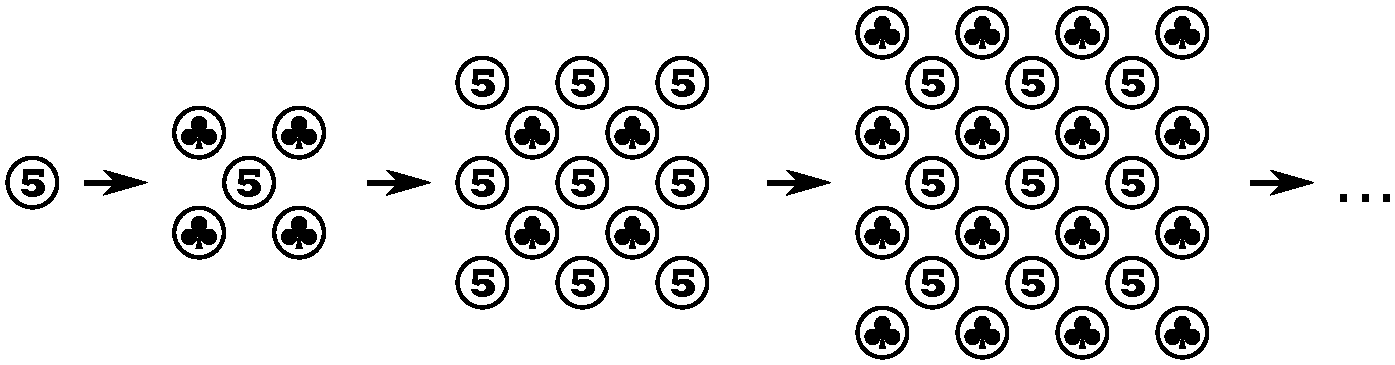
\includegraphics[width=.6\textwidth]{bilder/ZentrierteViereckszahlen.pdf}
\end{center}

\begin{aufgabe}{Der nächste Schritt}
	Erkennst du das Schema, nach dem ich dieses Muster gebaut habe? Kannst du das nächste Viereck zeichnen?
\end{aufgabe}

Während ich also immer größere Vierecke gelegt habe, ist mir das Folgende aufgefallen: Die Zahl an Münzen, die ich für ein Viereck benötige, scheint immer eine ungerade Zahl zu sein: Für das erste $1$, beim zweiten $5$, beim dritten $13$, beim vierten $25$, beim fünften \underline{\phantom{ 41 }}(?), \dots

Ob das wohl für alle solchen Vierecke stimmt? Ich habe noch ein paar weitere solcher Vierecke gelegt und tatsächlich habe ich für jedes eine ungerade Anzahl an Münzen gebraucht. Aber irgendwann sind mir natürlich die Münzen ausgegangen. Wie kann ich nun herausfinden, ob meine Vermutung wirklich für \emph{alle} solche Vierecke gilt?

Wir haben jetzt also für ein paar kleine Beispiele gesehen, dass die Aussage \glqq Für ein (zentriertes) Viereck benötigt man eine ungerade Zahl an Münzen.\grqq{} für diese stimmt. Wir können nun aber nicht \emph{alle} möglichen Vierecke durchprobieren und für jedes einzelne prüfen, ob die Aussage auch für diese stimmt.

Ein ähnliches Problem hatten wir zu Beginn dieses Schuljahres schon einmal in einem Zirkelbrief: Erinnerst du dich noch an den Brief mit den Unmöglichkeitsbeweisen? Die Tetrominos, Schachbretter und Chamäleons? 

\begin{center}
	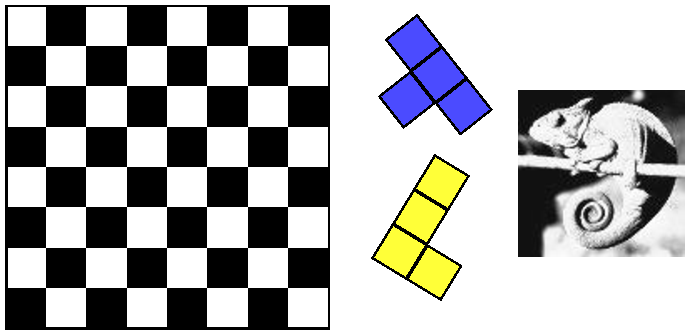
\includegraphics[width=.25\textwidth]{bilder/Erinnerung.pdf}
\end{center}

Darin hatten wir doch ein ganz ähnliches Problem: Wir hatten zum Beispiel eine Menge verschiedenfarbiger Chamäleons, die ihre Farbe nach einem bestimmten Muster ändern, wenn sie sich treffen. Wir wollten nun zeigen, dass wir nie gleich viele Chamäleons jeder Farbe bekommen können.

Dazu haben wir den Begriff einer \emph{Invariante} eingeführt: Eine Aussage, die ganz am Anfang wahr ist und die bei jedem Zwischenschritt (Treffen zweier Chamäleons) erhalten bleibt. Letzteres heißt: \emph{Vorausgesetzt} die Invariante gilt vor dem Treffen zweier Chamäleons, dann können wir daraus \emph{schließen}, dass sie auch nach dem Treffen wieder gilt. Dadurch wussten wir dann, dass diese Aussage zu \emph{jedem} Zeitpunkt gelten wird - und wir konnten daraus folgern, dass es nie gleich viele Chamäleons jeder Farbe geben wird.

Ganz ähnlich wollen wir nun auch mit unseren Münzvierecken vorgehen, um zu zeigen, dass wir immer eine ungerade Anzahl von Münzen benötigen:

\begin{description}
	\item[Anfang:] Für das kleinstmögliche Viereck (mit Seitenlänge $1$) ist die Aussage klar: Es besteht aus genau einer Münze - und $1$ ist eine ungerade Zahl.
	\item[Voraussetzung:] Wir haben ein Viereck mit Seitenlänge $n$, für das wir bereits wissen, dass wir ungerade viele Münzen benötigen um es zu legen.
	\item[Schlussfolgerung:] Wir wollen nun zeigen, dass auch ein Viereck mit Seitenlänge $n+1$ ungerade viele Münzen benötigt. Dazu nehmen wir unser Viereck mit Seitenlänge $n$ und machen daraus ein Viereck der Seitenlänge $n+1$:
	\begin{center}
		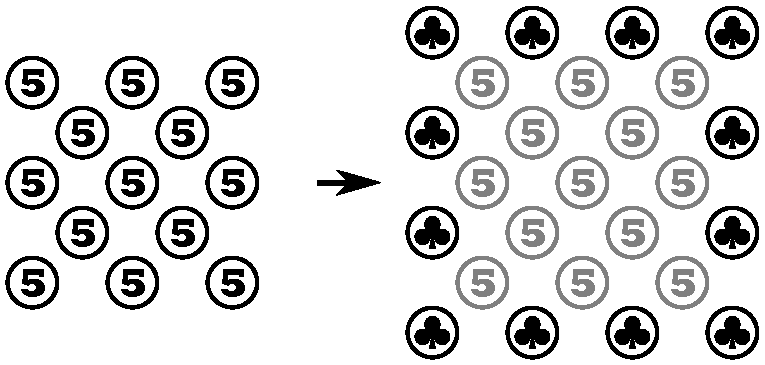
\includegraphics[width=.4\textwidth]{bilder/ZentrierteViereckszahlenBeweis.pdf}
	\end{center}
	Was müssen wir dazu also machen? Wir fügen auf jeder Seite zusätzlich eine Reihe Münzen hinzu $(\ast)$. Da wir dabei auf jeder der vier Seiten gleich viele Münzen hinzufügen, ist die Zahl der neuen Münzen sicher durch $4$ teilbar, also eine gerade Zahl.
	
	Die Gesamtzahl der Münzen im $(n+1)$-Viereck ist also gleich der Zahl der Münzen im $n$-ten Viereck (ungerade!) plus der Zahl der neuen Münzen (gerade!). Da die Summe einer geraden und einer ungeraden Zahl immer eine ungerade bildet
	\footnote{Du bist skeptisch, ob diese Aussage wirklich für alle Zahlen gilt? Sehr gut! In der Mathematik sollte man nie irgendwelche Behauptungen einfach so glauben, sondern sie am besten selbst nachprüfen. Teste die Aussage doch mal an einigen Beispielen. Wenn du sie wirklich beweisen willst, dann schau dir noch einmal den zweiten Korrespondenzbrief (zu Teilbarkeit) an - darin findest du alle dafür notwendigen Werkzeuge.},
	ist die Gesamtzahl der Münzen in unserem größeren Viereck erneut eine ungerade Zahl.
\end{description}

Damit haben wir nun bewiesen, dass \emph{alle} nach dem beschriebenen Schema gelegten Vierecke eine ungerade Anzahl von Münzen benötigen. Warum?

Nun, wenn wir ein Viereck mit irgendeiner beliebigen Seitenlänge (z.B. $n$) bauen wollen, dann können wir zunächst mal mit dem kleinstmöglichen Viereck beginnen (dem mit Seitenlänge $1$). Dafür benötigen wir eine ungerade Zahl an Münzen (nämlich eine) - das haben wir im Abschnitt \glqq Anfang\grqq{} gezeigt.

Dieses Viereck können wir nun schrittweise immer größer machen (erst zu einem mit Seitenlänge $2$, dann zu einem mit Seitenlänge $3$ usw.), bis wir bei der gewünschten Größe angekommen sind. Und wie wir oben gezeigt haben, kommt in jedem Schritt eine gerade Anzahl von Münzen hinzu. Hatten wir also vor einem Schritt eine ungerade Zahl Münzen verwendet (\glqq Voraussetzung\grqq ), so haben wir auch nach diesem Schritt insgesamt eine ungerade Anzahl Münzen benutzt (\glqq Schlussfolgerung\grqq ).

Insbesondere wissen wir damit, dass wir auch am Ende - wenn wir die gewünschte Größe erreicht haben - insgesamt eine ungerade Zahl Münzen verbaut haben.

\begin{aufgabe}{Wie viele neue Münzen?}
	Im obigen Beweis wird an der Stelle $(\ast)$ nur gesagt, dass die Zahl der neuen Münzen durch $4$ teilbar ist. Kannst du sogar herausfinden, wie viele Münzen es genau sind (in Abhängigkeit von $n$)?
	
	Anders gesagt: Wie viele zusätzliche Münzen benötigt man, um aus einen Viereck mit Seitenlänge $n$ eines mit Seitenlänge $n+1$ zu machen?
\end{aufgabe}

\begin{aufgabe}{Zentrierte Dreieckszahl}
	Natürlich kann man aus Münzen nicht nur Vierecke legen, sondern zum Beispiel auch Dreiecke:
	\begin{center}
		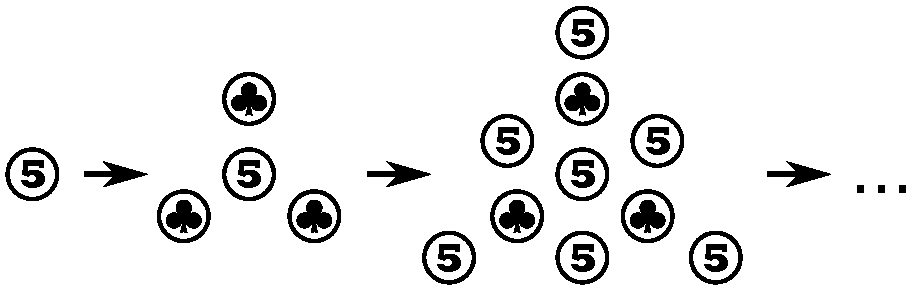
\includegraphics[width=.4\textwidth]{bilder/ZentrierteDreieckszahlen.pdf}
	\end{center}	
	Zeige, dass die die Zahl der dafür benötigten Münzen\footnote{Man bezeichnet diese Zahl übrigens auch als \glqq zentrierte Dreieckszahl\grqq{} - und entsprechend gibt es auch zentrierte Viereckszahlen, zentrierte Fünfeckszahlen usw.} nie durch $3$ teilbar ist (du kannst sogar noch genauer zeigen, dass sie immer um $1$ größer ist als eine durch $3$ teilbare Zahl).
\end{aufgabe}


\section{Induktion mit Zahlen}

Die Beweistechnik, die wir im vorangegangen Abschnitt kennengelernt haben, bezeichnet man als \emph{Beweis durch Induktion} oder \emph{Induktionsbeweis}. 

Mittels Induktion kann man Aussagen über \glqq Objekte\grqq{} beweisen, die folgende Eigenschaft haben: Es gibt unter ihnen ein oder mehrere \glqq kleinste\grqq{} Objekte und alle anderen Objekte können wir aus diesen kleinsten durch einen oder mehrere Zwischenschritte erhalten.

Ein Induktionsbeweis besteht dann aus folgenden drei Komponenten:

\begin{description}
	\item[Induktionsanfang (IA):] Wir beweisen die Aussage für das oder die kleinsten Objekte von Hand.
	\item[Induktionsvoraussetzung (IV):] Wir nehmen an, dass die zu zeigende Aussage für Objekte einer bestimmten Größe bereits gilt. Zunächst sind das nur die kleinsten Objekte (für die haben wir es ja im Induktionsanfang gezeigt). Nach einmaligem Anwenden des Induktionsschrittes gilt es auch für alle Objekte, die wir durch \emph{einen} Schritt aus einem kleinsten Objekt erhalten können. Dann für alle Objekte, die wir durch \emph{zwei} Schritte erhalten können, usw.
	\item[Induktionsschluss (IS):] Wir beweisen, dass die Aussage durch die Zwischenschritte, bei denen wir aus einem kleinen Objekt ein größeres machen, erhalten bleibt. Das heißt, wir zeigen das Folgende: Wann immer wir ein (kleines) Objekt haben, für das die Aussage gilt (d.h. die Induktionsvoraussetzung), und daraus mit einem Schritt ein größeres Objekt machen - \emph{dann} gilt die Aussage auch für dieses neue Objekt.
\end{description}


Einen natürlichen Kandidaten für Induktionsbeweise bildet nun die Menge der natürlichen Zahlen ($\mathbb{N} = \{1,2,3, \dots\}$). Denn diese hat ein kleinstes Objekt (die $1$) und alle anderen ihrer Elemente kann man aus diesem durch einen oder mehrere Zwischenschritte erhalten (nämlich ein- oder mehrmals $+1$ rechnen).
\footnote{Tatsächlich werden die natürlichen Zahlen in der Mathematik oft genau durch diese Eigenschaft definiert - nämlich über die \emph{Peano-Axiome}.}

Wann immer man also auf eine Aussage der Form \glqq Für alle natürlichen Zahlen $n \in \NN$ gilt \dots\grqq{} trifft, lohnt es sich auszuprobieren, ob man hier mit Induktion weiter kommt!

\begin{satz}\label{satz:zentrierteViereckszahl}
	Für alle natürlichen Zahlen $n$ gilt: $2n^2-2n$ ist eine durch $4$ teilbare Zahl.
\end{satz}

\begin{proof}
	Wir werden diese Aussage mittels Induktion zeigen:
	\begin{description}
		\item[IA ($n=1$):] $2n^2-2n  = 2\cdot 1^2 -2 \cdot 1 = 2-2 = 0$ ist durch $4$ teilbar.
		\item[IV (festes $n$):] Für festes $n$ sei $2n^2-2n$ durch $4$ teilbar.
		\item[IS ($n \to n+1$):] Wir wollen die Aussage für die Zahl $n+1$ zeigen unter der Voraussetzung, dass die Aussage für die nächstkleinere Zahl (also $n$) bereits gezeigt wurde. Und tatsächlich ist
		\[2(n+1)^2-2(n+1)  = 2n^2+4n+2-2n-2 = (2n^2-2n) + 4n\]
		durch $4$ teilbar, da es die Summe zweier durch $4$ teilbaren Zahlen ist - nämlich  $2n^2-2n$ (nach IV durch $4$ teilbar) und $4n$. \qedhere
	\end{description}
\end{proof}

\begin{aufgabe}{Eine Summenformel}\label{aufg:zentrierteDreieckszahl}
	Zeige mittels Induktion die folgende Behauptung:
	
	Für jede natürliche Zahl $n$ gilt:
	
	\[1 + 1\cdot3 + 2\cdot3 + \dots + (n-1)\cdot 3 = 1 + 3\cdot\frac{(n-1)\cdot n}{2}\] 
\end{aufgabe}

\begin{aufgabe}{Déjà-vu}\label{aufg:dejavu}
	Berechne $2n^2-2n+1$ für $n = 1,2,3,4,5$. Fällt dir etwas auf? (Schau am besten nochmal in den ersten Abschnitt!) 
	
	Kannst du deine Vermutung sogar beweisen? Evtl. geht das mit einem Induktionsbeweis, der einen Großteil der Struktur des Beweises von \Cref{satz:zentrierteViereckszahl} übernimmt.
	
	Zusatzfrage: Findest du einen ähnlichen Zusammenhang für die Zahl aus \cref{aufg:zentrierteDreieckszahl}?
\end{aufgabe}

\begin{aufgabe}{Induktion oder Nicht-Induktion?}
	Beweise: Für jede natürliche Zahl $n$ ist $2n^2-2n+1$ die Summe zweier direkt aufeinander folgender Quadratzahlen.
	
	Diese Aufgabe kannst du mit Induktion, aber auch direkt (durch Termumformung) zeigen. Wenn du \cref{aufg:dejavu} gelöst hast, kannst du die Behauptung hier sogar durch ein Bild zeigen!
	
	\emph{Hinweis:} Evtl. hilft es dir auch die Behauptung für ein paar kleine $n$ zu überprüfen - erkennst du dabei das allgemeine Muster?
\end{aufgabe}

\newpage

\section{Anwendungen der Induktion}

\subsection{Geometrisches}

Im letzten Korrespondenzbrief (zu Fraktalen) haben wir unter anderem die \emph{Kochsche Schneeflocke} betrachtet:
\begin{center}
	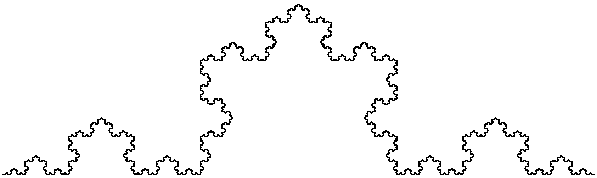
\includegraphics[width=.4\textwidth]{bilder/Schneeflocke-Konstruktion3.pdf}
\end{center}
Nur noch mal zur Erinnerung, wie man die Kochsche Schneeflocke (bzw. erstmal nur eine ihrer drei Seiten) erhält: Man beginnt mit einer einfachen Strecke. Diese Strecke teilt man in drei gleich lange Teile. Dann entfernt man das mittlere Stück und ersetzt es durch die zwei anderen Seiten eines gleichseitigen Dreiecks. Dadurch erhält man eine geometrische Figur, die aus vier Strecken besteht. Für den zweiten Schritt macht man nun mit jeder dieser vier Strecken das gleiche wie man es mit der ersten Strecke getan hat:
\begin{center}
	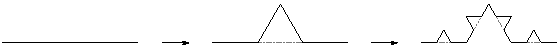
\includegraphics[width=.9\textwidth]{bilder/Schneeflocke-Konstruktion1.pdf}
\end{center}
Und das geometrische Objekt, das man \glqq nach unendlich vielen Schritten\grqq{} erhält, das nennt man dann Kochsche Schneeflocke.

Im letzten Korrespondenzbrief habe ich behauptet, dass die Länge der Linie, aus der die Kochsche Schneeflocke besteht, \emph{unendlich} lang ist. Der Beweis dazu war aber noch etwas ungenau: Wir haben nur gesehen, dass die Linie in den ersten beiden Schritten um jeweils mindestens \SI{1}{\cm} wächst - und dann einfach behauptet, dass das \glqq offensichtlich\grqq{} auch für alle weiteren Schritte so sein wird.

Jetzt aber haben wir die Technik des Induktionsbeweises kennen gelernt - und diese eignet sich perfekt um genau solche Argumente mathematisch präzise zu machen. 

\begin{satz}
	Beginnt man die Konstruktion einer Seite der Kochschen Schneeflocke mit einer Linie der Länge \SI{3}{\cm}, so ist die Linie nach dem $n$-ten Schritt mindestens $3+n$ \si{\cm} lang.
\end{satz}

Bevor du weiter liest: Kannst du dir so ungefähr vorstellen, wie der Induktionsbeweis für diese Aussage aussehen könnte? Was wird wohl der Induktionsanfang sein, was die Induktionsvoraussetzung und was der Induktionsschluss?

\begin{proof}
	Wir beweisen den Satz durch Induktion über $n$:
	\begin{description}
		\item[IA ($n=1$):] Nach dem ersten Schritt besteht die Linie aus $4$ Strecken, die jeweils einem Drittel der Anfangsstrecke entsprechen, also jeweils \SI{1}{\cm} lang sind. Die Gesamtlänge der Linie beträgt daher $4 \cdot \SI{1}{\cm} = \SI{4}{\cm} = 3+1\,\si{\cm}$.
		\item[IV:] Wir wissen für festes $n$: Nach dem $n$-ten Schritt hat die Linie die Länge $x$ \si{\cm}, wobei gilt $x \geq 3+n$.
		\item[IS ($n\to n+1$):] Im $(n+1)$-ten Schritt machen wir mit jeder Teilstrecke das gleiche, was wir im ersten Schritt mit der Anfangsstrecke gemacht haben. Dadurch wird also jede Strecke durch ein Linienstück ersetzt, das $\frac{4}{3}$-mal so lang ist. Dabei wird natürlich auch die Gesamtlinie um den Faktor $\frac{4}{3}$ gestreckt. Nach dem Schritt gilt also für die Gesamtlänge:
			\begin{align*}
			\text{Länge } 	&\geq \frac{4}{3}\cdot x\,\si{\cm} \overset{\text{\textbf{IV}}}{\geq} \frac{4}{3}\cdot (3+n)\,\si{\cm} = (4+\frac{4}{3}\cdot n)\,\si{\cm} > (4+ n)\,\si{\cm} \\
							&= (3+ (n+1))\,\si{\cm}
			\end{align*}
		Und das ist genau das, was wir zeigen wollten!
	\end{description}
\end{proof}

\begin{aufgabe}{Ein flächenloses Dreieck}
	Ein anderes Fraktal, welches wir im letzten Brief kennengelernt haben, war das Sierpinski-Dreieck: Es entsteht aus der Fläche eines gleichseitigen Dreiecks, indem man in jedem Schritt ein (oder später mehrere) kleinere Dreiecke aus ihm ausschneidet:
	\begin{center}
		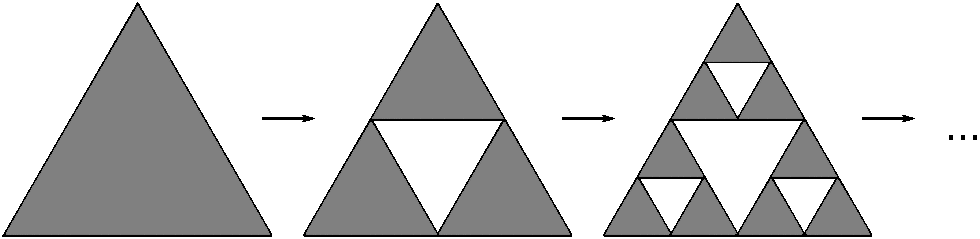
\includegraphics[width=.6\textwidth]{bilder/Sierpinski-Konstruktion.pdf}
	\end{center}
	Im Fraktalbrief wurde behauptet, dass die Fläche dieses Fraktals beliebig klein wird - und jetzt kannst du das auch beweisen! Zeige genauer die folgende Behauptung:
	\begin{satz}
		Hat das Dreieck zu Beginn eine Fläche von \SI{4}{\cm\squared}, so hat es nach $n$ Schritten eine Fläche von $\frac{9}{n+2}$ \si{\cm\squared} oder weniger.
	\end{satz}
	\emph{Erinnerung:} Im Fraktalbrief hatten wir bereits festgestellt, dass in jedem Schritt ein Viertel der grauen Fläche verloren geht. Hat man also vor dem Schritt eine Fläche von $x$ \si{\cm\squared}, so ist die Fläche danach noch $\frac{3}{4}\cdot x$ \si{\cm\squared}.
	
	\emph{Tipp:} Im Laufe des Beweises könnte eine Abschätzung der folgenden Form hilfreich sein: 
		\[\frac{\boxed{\phantom{123}}}{\boxed{\phantom{123}} + n} \leq \frac{\boxed{\phantom{123}}}{\boxed{\phantom{123}} + 1} \]
	wobei alles in den Boxen unverändert bleibt.
\end{aufgabe}


\subsection{Ein Abzählspiel}

Stell dir vor du bist im Mathe-Camp und möchtest mit einigen Freunden zusammen in einer kurzen Mathe-Pause Fußball spielen. Dazu müsst ihr nun festlegen, wer von euch der Team-Captain sein darf. Eine von euch schlägt nun das folgende Abzählverfahren vor um diese Person zu bestimmen:

Zunächst setzt ihr euch alle in einen Kreis. Dann beginnt eine von euch und tippt ihren linken Nachbarn an, der daraufhin den Kreis verlässt. Dessen Nachbar tippt nun wiederum seine linke Nachbarin an, die ebenfalls den Kreis verlässt, usw. Dieses Spiel spielt ihr, bis nur noch eine Person im Kreis übrig ist - diese ist dann der Team-Captain.

Für den Fall von $8$ Spielern, habe ich dir das Beispiel in \Cref{Abb:JosephusBsp} als Bild dargestellt:

\begin{figure}[h]\centering
	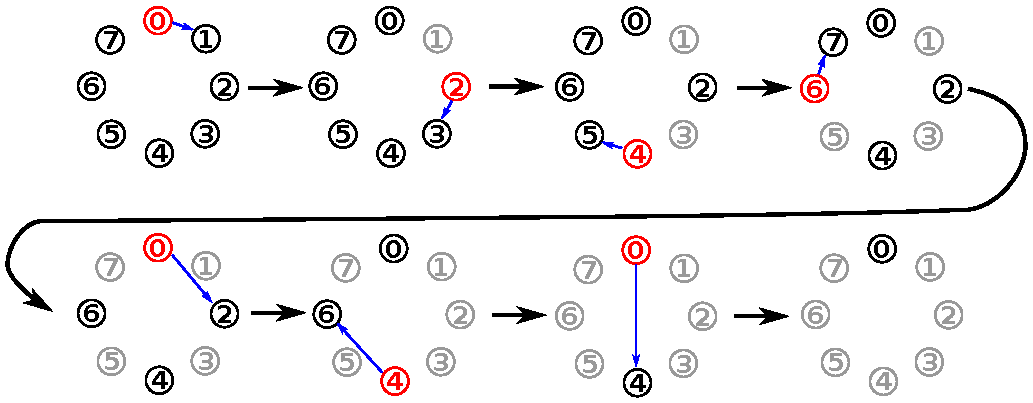
\includegraphics[width=\textwidth]{bilder/Josephus.pdf}
	\caption{Das Abzählverfahren für $8$ Personen. Die Person an der Reihe ist jeweils rot, der blaue Pfeil zeigt, wen sie antippt und graue Personen haben den Kreis bereits verlassen. Am Ende bleibt der Anfangsspieler ($0$) übrig.}
	\label{Abb:JosephusBsp}
\end{figure}

Wie du siehst, bleibt in diesem Fall also die Spielerin übrig, die auch angefangen hat. Ist das wohl immer so? Oder bleibt bei einer anderen Anfangszahl von Spielern auch manchmal jemand anders übrig? 

Diese Frage wollen wir nun genauer untersuchen! Um leichter über die verschiedenen Spieler reden zu können, habe ich diese mit Zahlen $0, 1, 2, \dots$ durchnummeriert. Und zwar beginnend mit dem Spieler, der das Abzählverfahren beginnt, und dann im Uhrzeigersinn den Kreis entlang.

\begin{frage}
	Verwendet eine Gruppe von $n$ Personen das oben beschriebene Abzählverfahren, welche Person bleibt dann am Ende übrig?
	\footnote{Diese Fragestellung ist auch als Josephus-Problem bekannt, benannt nach dem jüdischen Historiker Flavius Josephus (aus dem ersten Jahrhundert nach Christus).\footnote{Hilfe}}
\end{frage}

\begin{aufgabe}{Einige Beispiele}\label{aufgabe:JosephusBspe}
	Spiele das Verfahren einmal für verschiedene (kleine) Gruppengrößen durch und beobachte jeweils, welche Person am Ende übrig bleibt. Fülle dabei die folgende Tabelle aus:
	\begin{center}
		\renewcommand{\arraystretch}{2}\setlength{\tabcolsep}{1em}
		\begin{tabular}{l||c|c|c|c|c|c|c|c|c}
			Gruppengröße:	& 2	& 3 & 4 & 5 & 6 & 7 & 8 & 11 & 16 \\\hline
			Letzte Person:	&   &   &   &   &   &   & 0 &    &    
		\end{tabular}
	\end{center}
	Kannst du schon irgendein Muster erkennen? 
\end{aufgabe}

Nun wollen wir also ganz allgemein für alle möglichen Gruppengrößen zeigen, welche Person am Ende übrig bleibt. Und dafür bietet sich wieder einmal Induktion an. Kannst du dir schon vorstellen wie das in etwa ablaufen wird? Was könnte sich als Induktionsanfang eignen? Was als Induktionsschritt?

Zunächst einmal werden wir nur Gruppengrößen betrachten, die irgendeine $2$er-Potenz sind - warum das sinnvoll ist, wirst du gleich im Beweis sehen:

\begin{satz}\label{satz:Josephus1}
	Für alle natürlichen Zahlen $n$ gilt: Bei einer Gruppengröße von $2^n$ bleibt der Spieler $0$ am Ende übrig (also der, der anfängt).
\end{satz}

\begin{aufgabe}{Das Josephus-Problem für $2$er-Potenzen}
	Kannst du die Lücken im folgenden Induktionsbeweis für \Cref{satz:Josephus1} füllen?
	
	\begin{proof}
		Wir beweisen den Satz durch Induktion über $n$:
		\begin{description}
			\item[IA ($n=1$):] \textcolor{white}{Bei einer Gruppengröße von $2^1=2$ Personen ist lediglich ein einziger Spielzug notwendig: Spieler $0$ beginnt, indem er Spieler $1$ antippt. Dieser scheidet aus, wodurch Spieler $0$ als letzter Spieler übrig bleibt.}
			\item[IV:] Wir wissen für festes $n$: Bei einer Gruppe mit $2^n$ Personen bleibt am Ende der Spieler $0$ übrig.
			\item[IS ($n\to n+1$):] Wir haben nun also eine Gruppe aus $2^{n+1} = 2\cdot 2^n$ Spielern und wollen erneut zeigen, dass am Ende der Spieler $0$ übrig bleibt. Dazu starten wir das Verfahren und stoppen es, sobald zum ersten Mal wieder der Spieler $0$ an der Reihe ist. Folgende Spieler sind jetzt noch übrig:
			\[0, \underline{\phantom{2\quad}}, \underline{\phantom{4\quad}}, \underline{\phantom{6\quad}}, \underline{\phantom{8\quad}}, \dots , \underline{\phantom{ 2^{n+1}-2 }}\]
			Also gerade alle Spieler mit einer \underline{\phantom{ geraden\quad }} Nummer. Teilen wir jetzt die Nummer jedes verbliebenen Spielers durch $2$, so sind wir in der Anfangssituation des Abzählverfahrens für eine Gruppe mit \underline{\phantom{$2^n$\quad}} Spielern. Und für eine solche Gruppe wissen wir wegen der Induktionsvoraussetzung bereits, welcher Spieler am Ende übrig bleibt - nämlich Spieler \underline{\phantom{$0$\quad}}. \qedhere
		\end{description}
	\end{proof}
\end{aufgabe}

Jetzt wissen wir also, was passiert, wenn die Gruppe zufällig aus $2^n$ Spielern für irgendeine natürliche Zahl $n$ besteht. Was ist aber in den anderen Fällen? Nun, diese Fälle können wir nun einfach auf einen Fall zurückführen, für den wir die Lösung bereits kennen:

Angenommen unsere Gruppe besteht aus $2^n + k$ Personen (wobei $n$ und $k$ natürliche Zahlen sind und $k < 2^{n-1}$ gilt\footnote{Warum diese Einschränkung? Nun, damit möchte ich sicherstellen, dass während der ersten $k$ Spielzüge keine Person doppelt vorkommt (wie sorgt diese Einschränkung dafür?). Dadurch können wir in unserer weiteren Analyse immer davon ausgehen, dass wir noch im ersten Durchlauf des Kreises sind.}). Dann lassen wir das Verfahren einfach so lange laufen, bis noch $2^n$ Spieler übrig sind. Und in diesem Moment wissen wir, welcher Spieler übrig bleiben wird - nämlich genau der, der jetzt gerade an der Reihe ist.

\newpage
\begin{aufgabe}{Wer bleibt übrig?}
	Welcher Spieler bleibt nun übrig, wenn die Gruppe aus $2^n + k$ Personen besteht? Oder anders gefragt: Welcher Spieler ist an der Reihe, nachdem die ersten $k$ Spieler ausgeschieden sind?
	
	\emph{Hinweis:} Überlege dir die Antwort am besten erst einmal für ein paar kleine Beispiele: Welcher Spieler ist an der Reihe, nachdem der erste Spieler ausgeschieden ist? Wer ist dran, nachdem $2$ ausgeschieden sind? Wer, nachdem $3$ die Gruppe verlassen mussten? Kannst du jetzt ein Muster erkennen? Wenn du möchtest, kannst du deine Antwort wieder mit Hilfe einer einfachen Induktion (über $k$!) beweisen.
\end{aufgabe}

\begin{aufgabe}{Zur Kontrolle}
	Wenn wir keinen Fall vergessen haben, sollte es nun möglich sein, für jede denkbare Zahl an Spielern herauszufinden, wer bei dem Abzählverfahren am Ende übrig bleibt. Um das zu testen, versuche möglichst viele Felder der folgenden Tabelle auszufüllen (ohne das Verfahren, wie in \Cref{aufgabe:JosephusBspe} komplett durchzuspielen!):
	\begin{center}
	\renewcommand{\arraystretch}{2}\setlength{\tabcolsep}{1em}
	\begin{tabular}{l||c|c|c|c|c|c|c|c}
		Gruppengröße:	& 32 & 35 & 41 & 64 & 130 & 512 & 1025 & 2047 \\\hline
		Letzte Person:	&   &   &   &   &   &   &    &    
	\end{tabular}
	\end{center}	
	Möglicherweise ist es für diese Aufgabe hilfreich die ersten $2$er-Potenzen zu kennen: Diese sind:
		\[2, 4, 8, 16, 32, 64, 128, 256, 512, 1024, 2048, 4096, \dots \]
\end{aufgabe}


% Alternativer/Zusätzlich möglicher letzter Abschnitt: Korrektheitsbeweise
%Induktion verwendet man auch für Korrektheitsbeweise von Computerprogrammen:
%
%Beispiel: Quadratzahl $x^2$ berechnen als $x+x-1 +x-1+x-2 + \dots +1$ - evtl. dargestellt als Flussdiagramm (rekursives Programm!)
%
%Aufgabe?
%
%Euklidischer Algorithmus? Verweis auf zweiten Brief

\end{document}